\documentclass[xcolor=dvipsnames, 8pt]{beamer} %
%\setbeamertemplate{navigation symbols}{}

\usetheme{SantaBarbara}

\definecolor{black}{HTML}{0A0A0A}
\definecolor{green}{HTML}{0420eb} 
\definecolor{darkgreen}{HTML}{008000}
\definecolor{gold}{HTML}{FFD000}
\setbeamercolor{normal text}{fg=black,bg=white}
\setbeamercolor{alerted text}{fg=red}
\setbeamercolor{example text}{fg=black}
\setbeamercolor{palette primary}{fg=black, bg=gray!20}
\setbeamercolor{palette secondary}{fg=black, bg=gray!20}
\setbeamercolor{palette tertiary}{fg=white, bg=green!80}
\setbeamercolor{block title}{fg=black,bg=gold!40}
\setbeamercolor{frametitle}{fg=white, bg=green!80}
\setbeamercolor{title}{fg=white, bg=green!80}

\newcommand{\vecc}{\operatorname{vec}}
%\newcommand{\svec}{\operatorname{svec}}
\newcommand{\norm}[1]{\left| #1 \right|}
\newcommand{\xhat}{\hat{x}}
\newcommand{\uhat}{\hat{u}}
\newcommand{\yhat}{\hat{y}}
\newcommand{\wt}{\widehat{\theta}}

\usepackage[utf8]{inputenc}

\usepackage{tikz, tikzsettings}
\usepackage{verbatim}
\usepackage{amssymb}
\usepackage{amsmath}
%\usepackage{amsfonts}
\usepackage{algorithmic}
\graphicspath{{./}{./figures/}{./figures/presentation/}}
%\usepackage[version=4]{mhchem}
\usepackage{subcaption}
\usepackage[authoryear,round]{natbib}
%\usepackage{fancyvrb}
\usepackage{color}
\usepackage{colortbl}
\usepackage{xcolor}
\usepackage{physics}
\usepackage{pgfplots}
\usepackage{ragged2e}
%\pgfplotsset{compat=newest} 
%\pgfplotsset{plot coordinates/math parser=false}
%\usepackage{environ}
%\usetikzlibrary{decorations.markings}
%\usetikzlibrary{decorations.pathreplacing}
\usetikzlibrary{shapes,calc,spy, calc, backgrounds,arrows, fit, decorations.pathmorphing, decorations.pathreplacing, matrix}
%\usepackage[absolute,overlay]{textpos}
\usepackage{caption}
\usepackage{graphicx}
%\usepackage[controls=true,poster=first]{animate}

\newcommand{\useq}{\mathbf{u}}
\newcommand{\xseq}{\mathbf{x}}
\newcommand{\bbR}{\mathbb{R}}
\newcommand{\bbW}{\mathbb{W}}
\newcommand{\bbU}{\mathbb{U}}
\newcommand{\bbI}{\mathbb{I}}
\newcommand{\bbX}{\mathbb{X}}
\newcommand{\bbP}{\mathbb{P}}

\newcommand{\code}[1]{{\fontfamily{qcr}\selectfont#1}}

\AtBeginSection[]
{\frame<beamer>{\frametitle{Outline}   
	\tableofcontents[currentsection, currentsection]}
	\addtocounter{framenumber}{-1}}
	%
%{
%	\frame<beamer>{ 
%		\frametitle{Outline}   
%		\tableofcontents[currentsection,currentsubsection]}
		
%}

\makeatother
\setbeamertemplate{footline}
{
	\leavevmode%
	\hbox{%
		\begin{beamercolorbox}[wd=.3\paperwidth,ht=2.25ex,dp=1ex,center]{author in head/foot}%
			\usebeamerfont{author in head/foot}\insertshortauthor
		\end{beamercolorbox}%
		\begin{beamercolorbox}[wd=.6\paperwidth,ht=2.25ex,dp=1ex,center]{title in head/foot}%
			\usebeamerfont{title in head/foot}\insertshorttitle
		\end{beamercolorbox}%
		\begin{beamercolorbox}[wd=.1\paperwidth,ht=2.25ex,dp=1ex,center]{date in head/foot}%
			\insertframenumber{} / \inserttotalframenumber\hspace*{1ex}
	\end{beamercolorbox}}%
	\vskip0pt%
}


\title{Hybrid system identification using neural networks}
\date{Jan 19, 2021}
\author[Pratyush Kumar]{\large Pratyush Kumar}
\institute[UCSB]{
	\begin{minipage}{4in}
		\vspace{-10pt}
		\centering
		\raisebox{-0.1\height}{\includegraphics[width=0.25\textwidth]{UCSB_seal}}
		%\hspace*{.2in}
		%\raisebox{-0.5\height}{\includegraphics[width=0.25\textwidth]{jci_logo}}
	\end{minipage}
	\vspace{10pt}
	\newline
	{\large Department of chemical engineering}
	\vspace{10pt}
	\newline
	{\large Group talk}}

\begin{document}

%\frame{\titlepage}
	
\begin{frame}{Outline}
\tableofcontents
\end{frame}

\section{System identification}

\subsection{Koopman dynamic model}

\begin{frame}{Plant}
\begin{align*}
\dot x_p &= f_p(x_p, u, d, w) \\
y &= h_p(x_p) + v
\end{align*}

\begin{itemize}
	\setlength{\itemsep}{10pt}%
	\item $x_p \in \bbR^{n_p}$ (state), $y \in \bbR^{n_y}$ (measurement), 
	and $u \in \bbU$ (actuator), $d \in \bbR^{n_d}$ (disturbance). 
	\item $w \in \bbR^{n_w}$ (process noise), $v \in \bbR^{n_y}$ (measurement 
	noise).
	\item Goal: Obtain a dynamic model from data for subsequent use in 
	steady-state optimization or dynamic economic MPC.
\end{itemize}
\end{frame}

\begin{frame}{Black-box NN model}
\begin{align*}
\mathbf{y}_{k-N_p:k-1} &= [y(k-N_p)', y(k-N_p+1)', ..., y(k-1)']' \\
\mathbf{u}_{k-N_p:k-1} &= [u(k-N_p)', u(k-N_p+1)', ..., u(k-1)']' \\
z(k) &= [\mathbf{y}'_{k-N_p:k-1}, \mathbf{u}'_{k-N_p:k-1}]'
\end{align*}
in which, $N_p$ is the number of past inputs and outputs used.

\begin{align*}
x &= [y', z']' \\
x^+ &= \begin{bmatrix}
f_N(x, u, \theta_N) \\
y(k-N_p+1) \\
\vdots \\
y(k) \\
u(k-N_p+1) \\ 
\vdots \\
u(k)
\end{bmatrix} = f(x, u)\\
y &= [I, \ 0,\  0, \cdots]x = h(x)
\end{align*}

Note: Keeping the full state dynamics structure is helpful to make multi-step 
ahead forecasts.
\end{frame}

\begin{frame}{Koopman dynamic model}

Approach: Transform the state onto a manifold such that the system dynamics are 
approximately linear in that manifold \citep{korda:mezic:2018}.

\begin{align*} 
x_{kp} &= [y', z', f_N(y, z, \theta_N)']' \\
x_{kp}^+ &= Ax_{kp} + Bu = f(x, u)\\
y &= [I, \ 0] x_{kp} = h(x)
\end{align*}
	
\begin{itemize}
	\item $x_{kp} \in \bbR^N$, $f_N(\cdot)$ is a NN used for the nonlinear 
	transformation.
	\item Find $A$, $B$, and $\theta_N$ from data using the training 
	optimization problem.
\end{itemize}
\end{frame}

\subsection{Reactor example}


\begin{frame}{Nonlinear reactor model}
	
	\textbf{Plant}
	\begin{align*}
	\dfrac{dC_A}{dt} &= \dfrac{C_{Af} - C_A}{\tau} - k_1C_A\\
	\dfrac{dC_B}{dt} &= k_1C_A - 3k_2C^3_B + 3k_3C_C- \dfrac{C_B}{\tau}\\
	\dfrac{dC_C}{dt} &= k_2C^3_B - k_3C_C - \dfrac{C_C}{\tau}
	\end{align*}
	$u = C_{Af}$, $x = [C_A, C_B, C_C]'$.
	
\begin{itemize}
\item Assume full state feedback.
\item Use 18 hours (1080 samples) of training data, 6 hours (360 samples) of 
validation data.
\item Black-box NN architecture: $[3, \ 64, \ 3]$
\item Architecture of NN used in Koopman model lifting: $[3, \ 32, \ 32]$
\end{itemize}
\end{frame}

\begin{frame}{Model validation -- open loop data}
	\vspace{-0.1in}
	\begin{figure}
		\centering
		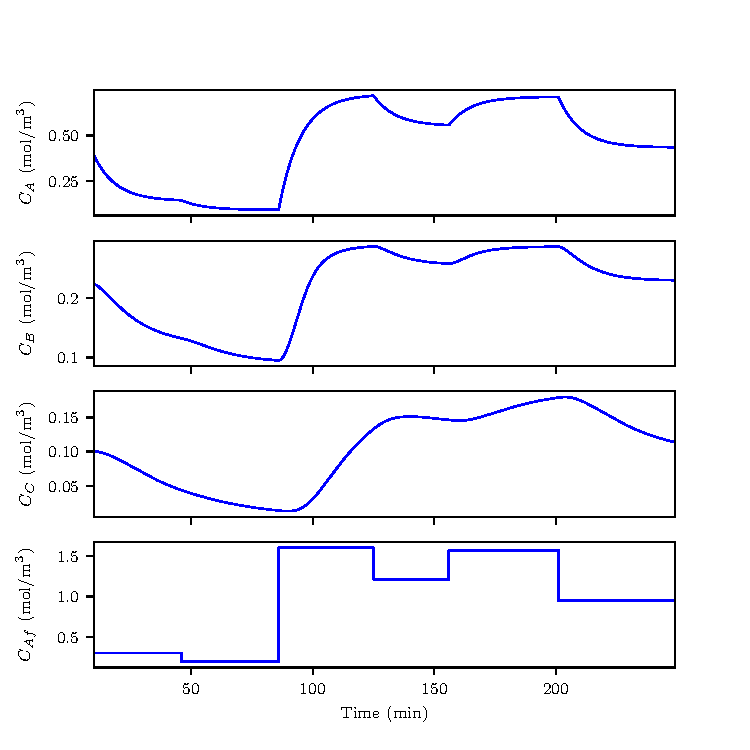
\includegraphics[page=1, height=0.8\textheight, 
		width=0.7\textwidth]{tworeac_plots.pdf}
	\end{figure}
\end{frame}

\begin{frame}{Steady-state optimization problem}
	\begin{align*}
	\underset{u_s}{\textnormal{min}} & \quad \ell(y_s, u_s) \\
	x_s &= f(x_s, u_s) \nonumber \\ 
	y_s &= h(x_s) \nonumber \\
	\underline{u} \leq &u_s \leq \overline{u} \nonumber
	\end{align*}
	
	For the reactor model, choose the stage cost as: $\ell(y_s, u_s) = 
	p_1C_{Afs} - p_2C_{Bs}$
	
\end{frame}

\begin{frame}{Steady-state cost curves}
	\begin{figure}
		\centering
		\includegraphics[page=1, height=0.7\textheight, 
		width=0.6\textwidth]{tworeac_ssopt.pdf}
	\end{figure}

\begin{itemize}
	\item The Koopman dynamic model has a linear structure, therefore, the cost 
	curve is linear as well. 
	\item The benefit of Koopman models, as discussed in 
	\cite{korda:mezic:2018} for tracking MPC, is that they would better 
	prediction accuracy than standard linear models.
\end{itemize}

\end{frame}

\section{Paresto}

\subsection{NLP setup with casadi}

\begin{frame}{Parameter estimation problem}

\begin{align*}
\underset{x(0), \theta}{\textnormal{min}} \sum_{k=0}^{N_t} 
\dfrac{1}{N_t} &\norm{\tilde{y}(k) - y(k)}^2_{R_v^{-1}}  \\
\textnormal{subject to} \quad \quad x^{+} &= f(x, u, \theta) \\
0 &= g(x, z, \theta) \\
\tilde{y} &= h(x, z, \theta)
\end{align*}

\begin{itemize}
	\setlength{\itemsep}{10pt}%
	\item Multi-step-ahead prediction-error minimization. 
	\item Multiple-shooting method: All the states ($x$ and $z$) 
	at each measurement instant are kept as decision variables in the 
	optimization. 
	\item The states are constrained by model equations, and states at each 
	time point are used to make forecasts at the next time point. 
	\item Confidence intervals are computed using Hessian of the objective. 
\end{itemize}
\end{frame}


\begin{frame}{Nonlinear programming in Casadi}
	
General NLP in Casadi
\begin{align*}
\underset{x}{\textnormal{min}} \quad &f(x, p) \\
\textnormal{subject to} \quad \underline{x} &\leq x \leq \overline{x} \\
\underline{g} &\leq g(x, p) \leq \overline{g}\\
\end{align*}

Casadi usage

\begin{center}
	
\code{nlpInfo = struct('x', x, 'f', fxp, 'g', gxp, 'p', p)} \\
\medskip
\code{testNlp = casadi.nlpsol('testNlp', 'solverName', nlpInfo, optsStruct)} \\
\medskip
\code{testNlp('x0', xguess, 'lbx', lbx, 'ubx', ubx, 'lbg', lbg, 'ubg', ubg, 
'p', pval)}
\end{center}

\begin{itemize}
	\item Now setup the previous parameter estimation problem in this format.
	\item The decision variable in the NLP as grey-box model parameters 
	($\theta$) and states ($x$ and $z$) at each time point, and parameters in 
	the NLP as measurements.
\end{itemize}
\end{frame}		

\begin{frame}{Problem setup}
	
Create casadi symbolics (decision variables, objective function, constraints, 
parameters). \\
\medskip

	\code{theta = casadi.MX.sym('theta', Ntheta);} \\
	\code{y = casadi.MX.sym('y', Ny*(Nt+1));}\\
	\code{xk = casadi.MX.sym('x0', Nx);}\\
	\code{zk = casadi.MX.sym('z0', Nz);}\\
	\code{w = \{ theta, x0, z0 \} \% decision variable list} \\
	\code{lsq = \{ y(1:Ny) - hxz('x', xk, 'z', zk, 'theta', theta) \}} \\
	\code{g = \{alg('x', xk, 'z', zk, 'theta', theta) \}} \\
	
	\medskip
	\code{for k=1:Nt} \\
	
	\medskip
	\code{\% Simulate via a casadi function.} \\
	\code{xkplus = fxz('x', xk, 'z', zk, 'theta', theta)}
	
	\medskip 
	\code{\% Create new decision variables.} \\
	\code{xk = casadi.MX.sym('xk', Nx);}\\
	\code{zk = casadi.MX.sym('zk', Nz);}\\
	\code{w\{end+1\} = xk;} \\
	\code{w\{end+1\} = zk;} \\
	
	\medskip 
	\code{\% Get objective function contribution.} \\
	\code{lsq\{end+1\} = y(k*Ny+1:(k+1)*Ny) - hxz('x', xk, 'z', zk, 'theta', 
	theta);} \\
	
	\medskip 
	\code{\% Get equality constraints.} \\
	\code{g\{end+1\} = xplus - xk;} \\
	\code{g\{end+1\} = alg('x', xk, 'z', zk, 'theta', theta);} \\
	
	\medskip
	\code{end\%for}

\end{frame}		

\begin{frame}{Create NLP solver and solve}
	
	\medskip
	
	\code{w = vertcat(w\{:\});} \\
	\code{J = sumsqr(lsq);} \\
	\code{g = vertcat(g\{:\});} \\
	\code{nlpInfo = struct('x', w, 'f', J, 'g', g, 'p', p)} \\
	\medskip
	\code{nlp = casadi.nlpsol('testNlp', 'ipopt', nlpInfo, optsStruct)} \\
	\medskip
	\code{nlp('x0', xguess, 'lbx', lbx, 'ubx', ubx, 'lbg', lbg, 'ubg', ubg, 
	'p', pval)} \\
	\medskip
	
An update needed in paresto: Handle data generated by time-varying control 
input profiles.
\end{frame}		

\subsection{KKT conditions and DAE bug}
\begin{frame}{KKT conditions}
	
Formulate Lagrangian \citep{andersson:rawlings:2018} - 
	
\begin{align*}
L(x, p, \lambda_x, \lambda_g) &= f(x, p) + \lambda_x' x + \lambda_g'g(x, p) \\
\lambda_x = \overline{\lambda}_x - \underline{\lambda}_x \\
\lambda_g = \overline{\lambda}_g - \underline{\lambda}_g \\
\end{align*}

KKT conditions - 
\begin{align*}
&\grad_x L(x, p, \lambda_x, \lambda_g) =0 \\
\underline{x} &\leq x \leq \overline{x} \\
\underline{g} &\leq g(x, p) \leq \overline{g} \\
&I^0_x \lambda_x + \overline{I}_x\overline{x} + \underline{I}_x\underline{x} - 
I_xx = 0 \\
&I^0_g \lambda_g + \overline{I}_g\overline{g} + \underline{I}_g\underline{g} - 
I_gg(x, p) = 0
\end{align*}

\begin{itemize}
	\item $\overline{I}_x$ and $\underline{I}_x$ are diagonal matrices with 
	zeros and ones denoting active and inactive constraints respectively.
	\item $I_x = \overline{I}_x + \underline{I}_x$ and $I^0_x = I - I_x$ denote 
	either and neither lower/upper bound active respectively.
	\item Casadi uses these active constraint informations to compute the 
	Hessian.
\end{itemize}

\end{frame}	

\begin{frame}{$\lambda = 0$ doesn't mean constraint is inactive}
	
Consider the following optimization problem - 
	
\begin{align*}
\underset{x, y}{\textnormal{min}} & \ (x-2)^2 \\
\textnormal{subject to} & x-y = 0
\end{align*}

Lagrangian - 
\begin{equation*}
	L(x, y, \lambda) = (x-2)^2 + \lambda (x-y)
\end{equation*}

KKT conditions - 
\begin{align*}
	2(x-2) + \lambda &= 0 \\
	-\lambda &= 0 \\
	x - y &= 0 \\
	\lambda &\geq 0 \\
	\lambda(x-y) &= 0
\end{align*}

\begin{itemize}
	\item Optimal solution is $x=y=2$ and $\lambda = 0$, but the equality 
	constraint is active. 
	\item Casadi was interpreting zero Lagrange multipliers as inactive 
	constraint, and therefore, was computing incorrect Hessian/confidence 
	intervals.
\end{itemize}




\end{frame}	

\begin{frame}{References}
\bibliographystyle{abbrvnat}
\bibliography{articles,proceedings,books,unpub}
\end{frame}

\end{document}
